\documentclass[11pt,a4paper]{article}
\usepackage[T1]{fontenc}
\usepackage{lmodern,amsmath,amssymb,amsthm,mathtools,booktabs,geometry,microtype}
\usepackage{xcolor}
\usepackage{tikz}
\usetikzlibrary{arrows.meta,positioning}
\usepackage[colorlinks=true,linkcolor=blue!45!black,citecolor=blue!45!black,urlcolor=blue!45!black]{hyperref}
\geometry{margin=25mm}
\newcommand{\E}{\mathbb E}
\newcommand{\R}{\mathbb R}
\newcommand{\Sset}{\mathcal S}
\newcommand{\Aset}{\mathcal A}
\newcommand{\one}{\mathbf 1}
\newtheorem{theorem}{Theorem}
\title{\textbf{Prometheus-RL}\\[4pt]\large Mathematical Foundations of a Reinforcement Learning Framework}
\author{Prometheus-RL Project}
\date{Technical manuscript v0.1.0 --- Phase 0}
\begin{document}
\maketitle
\begin{abstract}
We specify a research-oriented reinforcement learning framework, beginning with finite Markov decision processes and progressing to deep Q-learning for CartPole. The manuscript derives Bellman equations, establishes the contraction property underlying value iteration, explains temporal-difference learning and stochastic approximation, and develops the neural-network objective, replay memory, and target networks used by DQN. We distinguish mathematical guarantees in the tabular setting from empirical stabilization in deep learning. A concrete evaluation protocol and a modular implementation plan connect the mathematics to software. This is a design manuscript; no experiments or trained agents are reported at this stage.
\end{abstract}
\tableofcontents
\newpage
\section{The learning problem}
Supervised learning starts with target labels. Reinforcement learning instead seeks a policy whose sequence of decisions leads to favorable outcomes. Its central mathematical difficulty is that actions alter the distribution of future observations and rewards. A reward received much later may depend on an action taken now, creating a temporal credit-assignment problem. We follow the standard discounted formulation in \cite{sutton}.

At time $t$, the agent observes $S_t$, chooses $A_t$, receives $R_{t+1}$, and observes $S_{t+1}$. The policy is a conditional distribution $\pi(a\mid s)$, and the environment provides the dynamics. Figure~\ref{fig:loop} illustrates the separation of responsibilities.
\begin{figure}[ht]
\centering
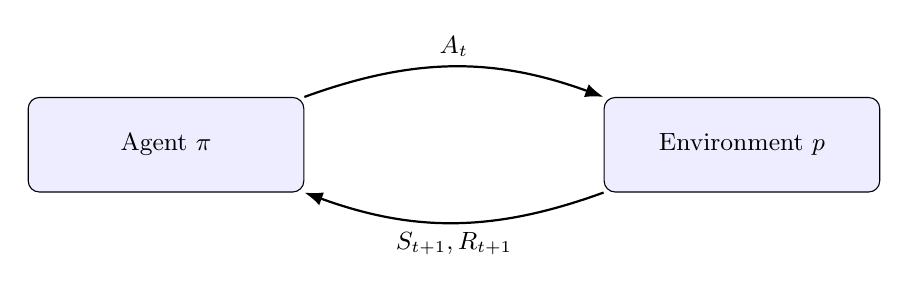
\begin{tikzpicture}[>=Latex,node distance=38mm,every node/.style={font=\small}]
\node[draw,rounded corners,fill=blue!7,minimum width=35mm,minimum height=12mm] (agent) {Agent $\pi$};
\node[draw,rounded corners,fill=blue!7,minimum width=35mm,minimum height=12mm,right=of agent] (env) {Environment $p$};
\draw[->,thick] (agent.north east) to[bend left=20] node[above] {$A_t$} (env.north west);
\draw[->,thick] (env.south west) to[bend left=20] node[below] {$S_{t+1}, R_{t+1}$} (agent.south east);
\end{tikzpicture}
\caption{The agent--environment feedback loop. The agent controls actions, not transitions or rewards.}\label{fig:loop}
\end{figure}

\section{Markov decision processes}
For the first implementation block we restrict ourselves to finite state and action spaces. An MDP is specified by
\[
\mathcal M=(\Sset,\Aset,p,\gamma,\mu_0),
\]
where $\mu_0$ is an initial-state distribution, $0\leq\gamma<1$ is a discount factor, and $p(s',r\mid s,a)$ is a joint probability kernel for the next state and reward. We assume bounded rewards and a finite reward support for the sums below. For continuous rewards or states the appropriate sums become integrals. For each legal $(s,a)$,
\[
 p(s',r\mid s,a)\geq 0,\qquad \sum_{s',r}p(s',r\mid s,a)=1.
\]
The Markov property is the conditional independence assertion
\[
 \Pr(S_{t+1},R_{t+1}\mid H_t,A_t)=p(S_{t+1},R_{t+1}\mid S_t,A_t),
\]
where $H_t$ denotes the observed history through $S_t$. The state must retain all predictive information needed for control; it need not be a literal description of every physical variable. Partial observability violates this assumption unless one can construct a suitable sufficient statistic, such as a belief state.

For a stationary policy, the probability of a finite trajectory $\tau=(s_0,a_0,r_1,s_1,\ldots,s_T)$ is
\[
 \Pr_\pi(\tau)=\mu_0(s_0)\prod_{t=0}^{T-1}\pi(a_t\mid s_t)p(s_{t+1},r_{t+1}\mid s_t,a_t).
\]
This factorization makes explicit which probabilities are controlled by the agent. We treat absorbing terminal states as having zero subsequent reward and a dummy action.

\subsection{Discounted return and the objective}
Define
\begin{equation}
 G_t=\sum_{k=0}^\infty\gamma^kR_{t+k+1}=R_{t+1}+\gamma G_{t+1}.
 \label{eq:return}
\end{equation}
For rewards satisfying $|R_t|\leq M$, absolute convergence follows from $|G_t|\leq M/(1-\gamma)$. The performance objective is $J(\pi)=\E_{\mu_0,\pi}[G_0]$. A finite episodic return may instead use $\gamma=1$ when termination and integrability justify it; the contraction proof below requires $\gamma<1$. Discounting is a modeling choice, not a universal requirement of rational decision-making.

\section{Value functions and Bellman equations}
Define the state and action values of a policy by
\begin{align*}
 V^\pi(s)&=\E_\pi[G_t\mid S_t=s],\\
 Q^\pi(s,a)&=\E_\pi[G_t\mid S_t=s,A_t=a].
\end{align*}
Applying conditional expectation to \eqref{eq:return} and using the Markov property yields
\begin{align}
 Q^\pi(s,a)&=\sum_{s',r}p(s',r\mid s,a)[r+\gamma V^\pi(s')],\\
 V^\pi(s)&=\sum_a\pi(a\mid s)Q^\pi(s,a).
\end{align}
These are consistency relations: a long-horizon expected return equals an immediate reward plus a discounted continuation. Define $r_\pi(s)=\sum_{a,s',r}\pi(a\mid s)p(s',r\mid s,a)r$ and $P_\pi(s,s')=\sum_{a,r}\pi(a\mid s)p(s',r\mid s,a)$. In vector form,
\begin{equation}
 V^\pi=r_\pi+\gamma P_\pi V^\pi,\qquad
 V^\pi=(I-\gamma P_\pi)^{-1}r_\pi.
\end{equation}
The inverse exists because $P_\pi$ is stochastic and the Neumann series $\sum_{k=0}^\infty\gamma^k P_\pi^k$ converges in the induced infinity norm. This gives an exact reference for small numerical tests.

\subsection{Optimality}
The optimal value is the supremum over policies. For finite discounted MDPs a stationary deterministic optimal policy exists. The Bellman optimality operator on action-value functions is
\begin{equation}
 (TQ)(s,a)=\sum_{s',r}p(s',r\mid s,a)\left[r+\gamma\max_b Q(s',b)\right].\label{eq:bellman}
\end{equation}
Its fixed point $Q^*$ induces a greedy optimal policy: $\pi^*(s)\in\arg\max_a Q^*(s,a)$. Ties may be broken arbitrarily. The following proof explains why iterating this operator is sound.

\begin{theorem}[Contraction of the Bellman optimality operator]
For any bounded action-value functions $Q,U$ on the finite MDP, $\|TQ-TU\|_\infty\leq\gamma\|Q-U\|_\infty$.
\end{theorem}
\begin{proof}
For any finite vectors $x,y$, $|\max_i x_i-\max_i y_i|\leq\max_i|x_i-y_i|$. Therefore, for each state-action pair,
\begin{align*}
 |(TQ)(s,a)-(TU)(s,a)|
 &\leq\gamma\sum_{s',r}p(s',r\mid s,a)\left|\max_bQ(s',b)-\max_bU(s',b)\right|\\
 &\leq\gamma\|Q-U\|_\infty\sum_{s',r}p(s',r\mid s,a)\\
 &=\gamma\|Q-U\|_\infty.
\end{align*}
Taking the maximum establishes the claim.
\end{proof}
By the Banach fixed-point theorem, $T$ has a unique fixed point and synchronous value iteration $Q_{k+1}=TQ_k$ obeys
\[
 \|Q_k-Q^*\|_\infty\leq\gamma^k\|Q_0-Q^*\|_\infty.
\]
To see optimality, choose a greedy policy at the fixed point. Its policy Bellman operator agrees with $T$ there, so the fixed point equals its policy value. Every other policy has an operator bounded above by $T$ at that fixed point; monotonicity and contraction imply its value cannot exceed it. The Bellman residual also bounds the error:
\[
 \|Q-Q^*\|_\infty\leq\frac{\|TQ-Q\|_\infty}{1-\gamma}.
\]
These properties will supply both a stopping criterion and test oracles for block 1.

\subsection{Worked example: delayed reward}
Consider states $s_0,s_1$ and an absorbing terminal state. At $s_0$, action \emph{cash} terminates for reward 2, while \emph{wait} moves deterministically to $s_1$ for reward 0. At $s_1$ the only action terminates for reward 5. With $\gamma=0.9$,
\[
 Q^*(s_0,\text{cash})=2,\quad Q^*(s_1,\text{collect})=5,\quad
 Q^*(s_0,\text{wait})=0.9(5)=4.5.
\]
Beginning at $Q_0=0$, the first Bellman iteration learns the immediate rewards; the second propagates 5 backward. A greedy policy on immediate reward alone chooses cash, but a greedy policy on optimal action values chooses wait. This example will be encoded as an analytic regression test.

\section{Temporal-difference learning and Q-learning}
Value iteration assumes a known transition kernel. In model-free learning the agent instead observes transitions $e_t=(s_t,a_t,r_{t+1},s_{t+1},d_t)$, with $d_t=1$ for true termination. In TD(0) policy evaluation, the temporal-difference error is
\[
 \delta_t=r_{t+1}+\gamma(1-d_t)V(s_{t+1})-V(s_t),
 \qquad V(s_t)\leftarrow V(s_t)+\alpha_t\delta_t.
\]
A bootstrap target combines a measured reward with the current estimate of a future value. Q-learning \cite{watkins} uses the optimality operator rather than a policy-expectation operator:
\begin{align}
 y_t&=r_{t+1}+\gamma(1-d_t)\max_b Q_t(s_{t+1},b),\\
 Q_{t+1}(s_t,a_t)&=Q_t(s_t,a_t)+\alpha_t[y_t-Q_t(s_t,a_t)].\label{eq:qlearn}
\end{align}
All other table entries are unchanged. Conditional on the present estimate and sampled state-action pair, the expected target is $(TQ_t)(s_t,a_t)$, under the MDP kernel. Thus the expected update points toward the Bellman fixed point, while the observed reward and transition introduce sampling noise. This is stochastic approximation rather than exact dynamic programming.

\subsection{Convergence and exploration}
For a finite stationary discounted MDP with bounded rewards, tabular Q-learning converges almost surely to $Q^*$ under the usual sufficient exploration and step-size conditions \cite{watkins,sutton}. In particular every state-action pair must be sampled infinitely often, with per-pair step sizes satisfying
\[
 \sum_{n=1}^\infty\alpha_n(s,a)=\infty,\qquad
 \sum_{n=1}^\infty\alpha_n(s,a)^2<\infty.
\]
The first condition prevents learning from stopping too early; the second controls accumulated noise. A constant step size is practical but does not meet this convergence theorem. With one chosen greedy action $a^*$ and $m$ legal actions, an epsilon-greedy behavior policy is
\[
 \pi_\epsilon(a\mid s)=\frac{\epsilon}{m}+(1-\epsilon)\one_{\{a=a^*\}}.
\]
It mixes random exploration and exploitation. Q-learning is off-policy: the target uses greedy continuation even when the behavior explores. An epsilon schedule alone does not guarantee that every state-action pair will be visited infinitely often.

For example, with $Q(s,a)=2$, reward 1, next maximum 4, $\gamma=0.9$ and $\alpha=0.1$, the target is $4.6$, TD error is $2.6$, and the new entry is $2.26$. For true termination the same transition instead gives target 1 and new entry $1.9$.

\section{Deep Q-networks}
A table is impractical for high-dimensional or continuous state spaces. DQN \cite{mnih} approximates the action-value vector by a network $f_\theta:\R^n\to\R^m$, with one output for each discrete action. For CartPole the proposed baseline uses $n=4$, $m=2$, and two fully connected hidden layers of width 128:
\begin{align*}
 h_1&=\operatorname{ReLU}(W_1s+b_1),& W_1&\in\R^{128\times4},\\
 h_2&=\operatorname{ReLU}(W_2h_1+b_2),& W_2&\in\R^{128\times128},\\
 f_\theta(s)&=W_3h_2+b_3,& W_3&\in\R^{2\times128}.
\end{align*}
The output is linear, not a softmax: Q-values represent expected returns and need not be probabilities or sum to one. The architecture contains $640+16512+258=17410$ trainable parameters. For a minibatch of size $B$, the network yields a $B\times m$ tensor; gather the action column for each transition to obtain $B$ predictions.

\subsection{The loss and semi-gradient}
The online network has parameters $\theta$; a second network has parameters $\bar\theta$. Given a batch of transitions, define
\begin{align}
 y_i&=r_i+\gamma(1-d_i)\max_b Q_{\bar\theta}(s'_i,b),\label{eq:target}\\
 L(\theta)&=\frac1B\sum_{i=1}^B \ell(Q_\theta(s_i,a_i)-y_i).
\end{align}
For squared loss $\ell(u)=u^2/2$, differentiation with the targets held fixed gives
\[
 \nabla_\theta L=\frac1B\sum_i(Q_\theta(s_i,a_i)-y_i)\nabla_\theta Q_\theta(s_i,a_i).
\]
Gradient descent updates $\theta\leftarrow\theta-\eta\nabla_\theta L$. The target is detached from automatic differentiation; this is a semi-gradient method when the target ultimately depends on the learned value function. We propose Huber loss for the baseline,
\[
 \ell_\kappa(u)=\begin{cases}u^2/2&|u|\leq\kappa,\\
 \kappa(|u|-\kappa/2)&|u|>\kappa,\end{cases}
\]
with $\kappa=1$. Its derivative is bounded, reducing sensitivity to large TD errors. We will use Adam as an adaptive optimizer, with all hyperparameters recorded. A finite-difference test can check the loss gradient on a small fixed-target network away from ReLU kinks.

\subsection{Replay and target synchronization}
A replay buffer stores recent experiences and samples minibatches, reducing short-range temporal correlation and permitting reuse of data. Samples are not perfectly independent draws from the stationary state distribution: the buffer is finite and reflects multiple historical policies. At intervals of $C$ environment steps we propose hard synchronization $\bar\theta\leftarrow\theta$. Between synchronizations the bootstrap target is more stationary. The network, replay and target copy are separate modules to make unit tests meaningful.

Deep off-policy learning combines bootstrapping, function approximation, and off-policy sampling. This combination can be unstable; the tabular contraction theorem does not transfer to the learned neural projection. Replay and target networks are empirical stabilization techniques, not a proof of convergence.

\begin{figure}[ht]
\centering
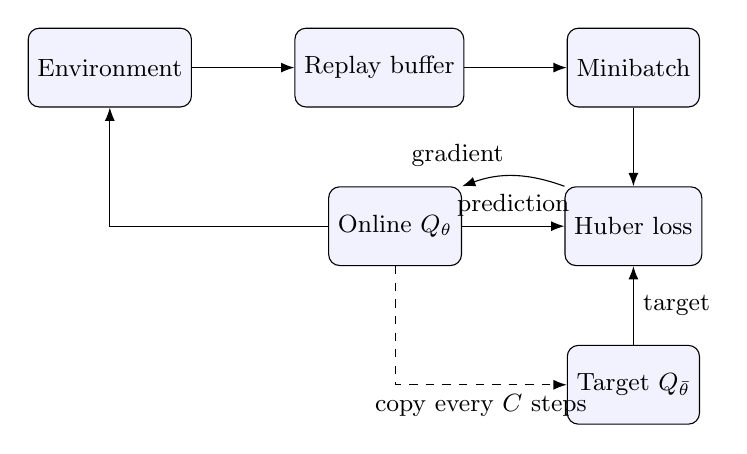
\begin{tikzpicture}[>=Latex,node distance=10mm and 13mm,every node/.style={font=\small},box/.style={draw,rounded corners,align=center,minimum height=10mm,fill=blue!5}]
\node[box] (env) {Environment};
\node[box,right=of env] (buf) {Replay buffer};
\node[box,right=of buf] (batch) {Minibatch};
\node[box,below=of batch] (loss) {Huber loss};
\node[box,left=of loss] (online) {Online $Q_\theta$};
\node[box,below=of loss] (target) {Target $Q_{\bar\theta}$};
\draw[->] (env)--(buf); \draw[->] (buf)--(batch); \draw[->] (batch)--(loss);
\draw[->] (online)--node[above]{prediction}(loss);
\draw[->] (target)--node[right]{target}(loss);
\draw[->] (loss.north west) to[bend right=20] node[above left]{gradient} (online.north east);
\draw[->,dashed] (online.south) |- node[pos=.75,below]{copy every $C$ steps} (target.west);
\draw[->] (online.west) -| (env.south);
\end{tikzpicture}
\caption{Proposed DQN architecture. The target network does not receive optimizer gradients.}\label{fig:dqn}
\end{figure}

\section{CartPole as a control problem}
CartPole is an inverted pendulum on a movable cart. Its observation is $s=(x,\dot x,\phi,\dot\phi)$, with position, velocity, pole angle relative to upright and angular velocity. Actions apply a fixed horizontal force in either direction. Under the ideal frictionless cart-pole model used in the classic Gymnasium implementation \cite{gymcart}, write $M=m_c+m_p$, $l$ for the pole half-length, and $F$ for force. Define
\begin{align*}
 z&=\frac{F+m_pl\dot\phi^2\sin\phi}{M},\\
 \ddot\phi&=\frac{g\sin\phi-z\cos\phi}{l(4/3-m_p\cos^2\phi/M)},\\
 \ddot x&=z-\frac{m_pl\ddot\phi\cos\phi}{M}.
\end{align*}
With Euler integration over time step $\Delta t$, the position and angle advance by their old velocities multiplied by $\Delta t$, and velocities advance by the corresponding accelerations. Near upright, $\sin\phi\approx\phi$ and $\cos\phi\approx1$. With $F=0$ the leading angular acceleration is $g\phi/[l(4/3-m_p/M)]$, which has the same sign as the deviation. The upright equilibrium is unstable. The agent must learn to correct the deviation using the reward feedback rather than explicit equations of motion.

In CartPole-v1 the standard reward is +1 per step, including the terminating step, with the default time limit of 500 steps. A failure occurs when the cart or pole leaves the permitted range. The undiscounted episodic return counts survived steps, whereas discounted return emphasizes near-term survival.

\subsection{Termination versus truncation}
Gymnasium returns separate termination and truncation flags \cite{gymtime}. A true terminal transition has no future task reward, so $d=1$ in \eqref{eq:target}. An externally imposed time limit usually truncates a continuing task; the state remains meaningful and the target still bootstraps with $d=0$. Both flags end the collection episode, but only true termination removes the bootstrap term in this setting. A genuine finite-horizon objective is different: include time remaining in the state and use zero continuation at its horizon. The collector must preserve the final observation before resetting the environment.

\section{Extensions and the research program}
\subsection{Double DQN}
If $X_a$ are unbiased noisy estimates of fixed action values $q_a$, Jensen's inequality gives $\E[\max_a X_a]\geq\max_a q_a$. For example, if two true values are zero and independent estimates are each uniformly $+1$ or $-1$, the maximum equals $-1$ only with probability $1/4$, so its expectation is $1/2$. Double DQN \cite{double} reduces this coupling by choosing with the online network and evaluating with the target network:
\[
 y=r+\gamma(1-d)Q_{\bar\theta}(s',\arg\max_b Q_\theta(s',b)).
\]
This can reduce overestimation but cannot guarantee unbiased estimates because the two networks are correlated.

\subsection{Dueling networks and prioritized replay}
A dueling network \cite{dueling} separates state value and relative action advantages. One common aggregation is
\[
 Q(s,a)=V(s)+A(s,a)-\frac1m\sum_b A(s,b).
\]
Subtracting mean advantage makes the advantage offset irrelevant to the output and ensures $V$ is the mean output Q-value of the architecture (not necessarily the value of an arbitrary policy). Prioritized replay \cite{per} uses priority $p_i=|\delta_i|+\varepsilon$ and sampling probabilities $P(i)=p_i^\alpha/\sum_jp_j^\alpha$. Importance weights $(NP(i))^{-\beta}$ partially correct the changed sampling distribution for $N$ stored transitions; full correction of the uniform-buffer expectation uses $\beta=1$ with unnormalized weights, under fixed priorities and losses. We will compare these extensions individually rather than confound their effects.

\subsection{Beyond value-based control}
For differentiable policies, define $J(\theta)=\E_{\tau\sim\pi_\theta}[G_0]$. In a finite episodic task, differentiating the trajectory probability and dropping past rewards by conditional expectation yields the score-function identity
\[
 \nabla_\theta J=\E\left[\sum_t\gamma^t G_t\nabla_\theta\log\pi_\theta(A_t\mid S_t)\right].
\]
A state-dependent baseline can reduce variance without changing the expectation, since
\[\E_{a\sim\pi}[\nabla_\theta\log\pi_\theta(a\mid s)]=0.\]
PPO \cite{ppo} is planned after the DQN family; its clipped probability-ratio objective will be derived in a later version.

\section{Experimental design and implementation contracts}
\subsection{Proposed baseline configuration}
Table~\ref{tab:params} gives starting settings, not experimentally optimized parameters. We will log training interactions, elapsed time, losses, evaluation return and failure rates. Evaluation must not update parameters or replay.
\begin{table}[ht]
\centering
\caption{Initial DQN hyperparameter proposal.}\label{tab:params}
\begin{tabular}{ll@{\quad}ll}
\toprule
Parameter & Value & Parameter & Value\\
\midrule
Discount $\gamma$ & 0.99 & Batch size & 64\\
Adam learning rate & $10^{-3}$ & Replay capacity & 50,000\\
Warmup & 1,000 steps & Target copy period & 500 steps\\
Exploration & 1.0 to 0.05 & Decay duration & 20,000 steps\\
Training budget & 100,000 steps & Device & CPU first\\
\bottomrule
\end{tabular}
\end{table}

\subsection{Evaluation and uncertainty}
The independent experimental unit is a training seed, not an episode. Use five independent training seeds initially, 100 separate evaluation episodes per trained agent, and compare to a random-action baseline using the same episode budget. For seed $j$, let $\bar R_j=\frac1{100}\sum_{i=1}^{100}R_{ji}$. Report all five means, their overall mean $\bar R=\frac15\sum_j\bar R_j$ and sample standard deviation. A Student-$t$ interval can be reported cautiously with five seeds if its approximate normality assumptions are plausible; do not treat the 500 correlated within-agent observations as 500 independent training runs. Proposed success criterion: every agent has held-out mean return at least 475 out of 500. If this fails, publish the negative result and revise the configuration in a new, traceable experiment. Hyperparameter selection uses validation seeds separate from final test seeds.

Reproducibility requires the commit hash, package versions, environment ID, device, training budget, configuration and all random seeds. Seed Python, NumPy, PyTorch, environment resets and action sampling as appropriate. Hardware and library nondeterminism may remain; seed control is not a guarantee of bitwise equality.

\subsection{Software contracts}
The finite MDP layer validates transition probabilities and exposes Bellman operators; the tabular agent implements \eqref{eq:qlearn}; the replay layer stores transition data including both episode-end flags; the network layer maps batched observations to action values; the DQN agent implements \eqref{eq:target} and the semi-gradient update; the training loop manages interaction budgets and evaluation. Each contract has an associated test: analytic Bellman solutions, terminal masking, replay capacity and seed behavior, tensor dimensions, target immutability, and held-out evaluation. We will retain small deterministic tests even after adding stochastic experiments.

\section{Conclusion and current limitations}
The central algorithmic progression is from exact Bellman operators to stochastic tabular updates and then to neural approximations. The rigorous guarantees apply to their stated mathematical assumptions, whereas deep Q-learning must be evaluated empirically. Phase 0 establishes project packaging, Git workflow, CI, and this mathematical specification. No learning algorithms are implemented yet, the proposed settings are unvalidated, and all training benchmarks remain future work. Each subsequent pull request will update both implementation and manuscript so that mathematical claims remain aligned with code and observed results.

\begin{thebibliography}{9}
\bibitem{sutton} R. S. Sutton and A. G. Barto. \emph{Reinforcement Learning: An Introduction}, 2nd ed., MIT Press, 2018. \url{http://incompleteideas.net/book/the-book-2nd.html}.
\bibitem{watkins} C. J. C. H. Watkins and P. Dayan. Q-learning. \emph{Machine Learning}, 8:279--292, 1992. \url{https://doi.org/10.1007/BF00992698}.
\bibitem{mnih} V. Mnih et al. Human-level control through deep reinforcement learning. \emph{Nature}, 518:529--533, 2015. \url{https://doi.org/10.1038/nature14236}.
\bibitem{double} H. van Hasselt, A. Guez, and D. Silver. Deep reinforcement learning with double Q-learning. AAAI, 2016. \url{https://arxiv.org/abs/1509.06461}.
\bibitem{dueling} Z. Wang et al. Dueling network architectures for deep reinforcement learning. ICML, 2016. \url{https://arxiv.org/abs/1511.06581}.
\bibitem{per} T. Schaul et al. Prioritized experience replay. ICLR, 2016. \url{https://arxiv.org/abs/1511.05952}.
\bibitem{ppo} J. Schulman et al. Proximal policy optimization algorithms. 2017. \url{https://arxiv.org/abs/1707.06347}.
\bibitem{gymcart} Farama Foundation. Gymnasium CartPole implementation. \url{https://github.com/Farama-Foundation/Gymnasium/blob/main/gymnasium/envs/classic_control/cartpole.py}.
\bibitem{gymtime} Farama Foundation. Handling time limits. Gymnasium documentation. \url{https://gymnasium.farama.org/tutorials/gymnasium_basics/handling_time_limits/}.
\end{thebibliography}
\end{document}
